\section{Experimental Results}
\label{sec:experiments}

\subsection{Setup}
\label{sec:setup}

\textbf{Data.}
We train on the 1865 training pairs of the SID Sony subset~\cite{chen2018sid} (Sony
$\alpha$7S\,II) and test on its 236 test pairs with exposure ratio $\times300$, at full
resolution. Several noisy shots of a scene share one long-exposure reference.

\textbf{Training.}
Each model trains for 10 epochs on one NVIDIA A40 (48\,GB), with $1200\times1200$ random crops,
batch size 1 and bf16 autocast. We use Adam with learning rate $2.5\times10^{-4}$ for the context
processor and region attention (including the illumination layers), and $5\times10^{-5}$ for the
rest of the U-Net. The paper also fine-tunes the residual VAE in a first stage; at about two hours
per epoch this was too slow for us, so all models share the pretrained SD VAE with zero-initialised
skips. \sdtwo{} is trained as in DarkDiff; the three compact backbones are trained with
illumination-aware conditioning.

\textbf{Metrics.}
We report PSNR and SSIM~\cite{wang2004ssim} on $[0,1]$ images and LPIPS~\cite{zhang2018lpips}
with AlexNet features. For efficiency we report trainable parameters (U-Net, context processor
and new layers), U-Net GFLOPs per call, inference time and peak memory per image (50 DDIM steps
with CFG), and time and peak memory per training step.

\textbf{Scope.}
The paper trains for 3000 epochs on eight A100 GPUs, on SID and LRD, and evaluates on SID, ELD
and LRD. Our budget is 0.3\% of those epochs on one GPU, so our numbers compare the backbones with
each other at equal budget. They are not comparable with the published scores.

\subsection{Image Quality}
\label{sec:quality}

\begin{table}[t]
  \centering
  \caption{Image quality on the SID $\times300$ test set after 10 epochs.
  $\uparrow$: higher is better; $\downarrow$: lower is better. Best of our runs in bold.}
  \label{tab:quality}
  \setlength{\tabcolsep}{5pt}
  \begin{tabular}{@{}lccc@{}}
    \toprule
    Model & PSNR (dB) $\uparrow$ & SSIM $\uparrow$ & LPIPS $\downarrow$ \\
    \midrule
    \sdtwo{} (DarkDiff, baseline) & \textbf{8.36} & 0.253          & 0.879 \\
    \bksdm{} + illum.             & 7.42          & \textbf{0.307} & 0.813 \\
    \sdxs{} + illum.              & 6.55          & 0.286          & 0.800 \\
    \tinysd{} + illum.            & 4.36          & 0.296          & \textbf{0.776} \\
    \midrule
    \textcolor{gray}{DarkDiff~\cite{zheng2025darkdiff}, 3000 ep.} &
    \textcolor{gray}{26.78} & \textcolor{gray}{0.644} & \textcolor{gray}{0.186} \\
    \bottomrule
  \end{tabular}
\end{table}

Table~\ref{tab:quality} gives the results. All models are far from convergence: the
published DarkDiff model reaches 26.78\,dB and an LPIPS of 0.186 after its full run. Even so,
the ranking is informative. All three compact, illumination-guided models beat the \sdtwo{}
baseline on both SSIM and LPIPS. \bksdm{} has the best SSIM (0.307, +21\%) and \tinysd{} the
best LPIPS (0.776, $-12\%$). PSNR ranks the models in the opposite order. When outputs are this
far from the target, PSNR is dominated by global brightness and colour errors, and the compact
models produce over-bright images with colour casts. SSIM and LPIPS respond to structure, and
they agree with our visual ranking.

\begin{figure*}[t]
  \centering
  \setlength{\tabcolsep}{1.5pt}
  \begin{tabular}{ccc}
    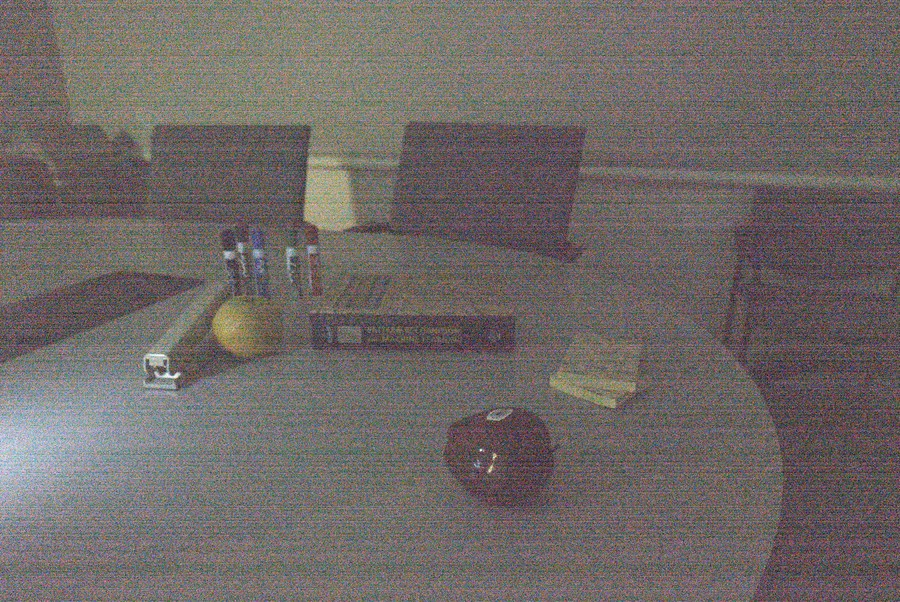
\includegraphics[width=0.32\linewidth]{input} &
    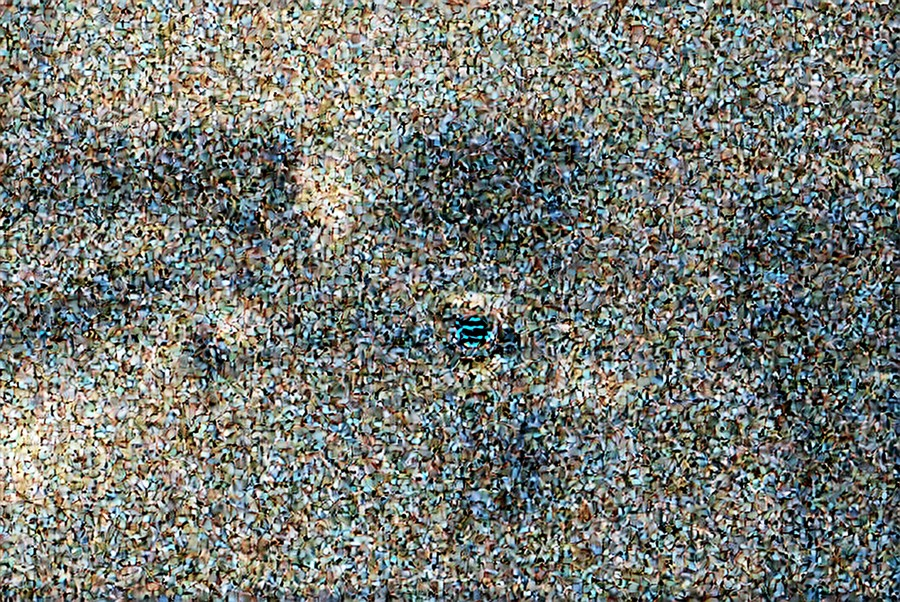
\includegraphics[width=0.32\linewidth]{sd21} &
    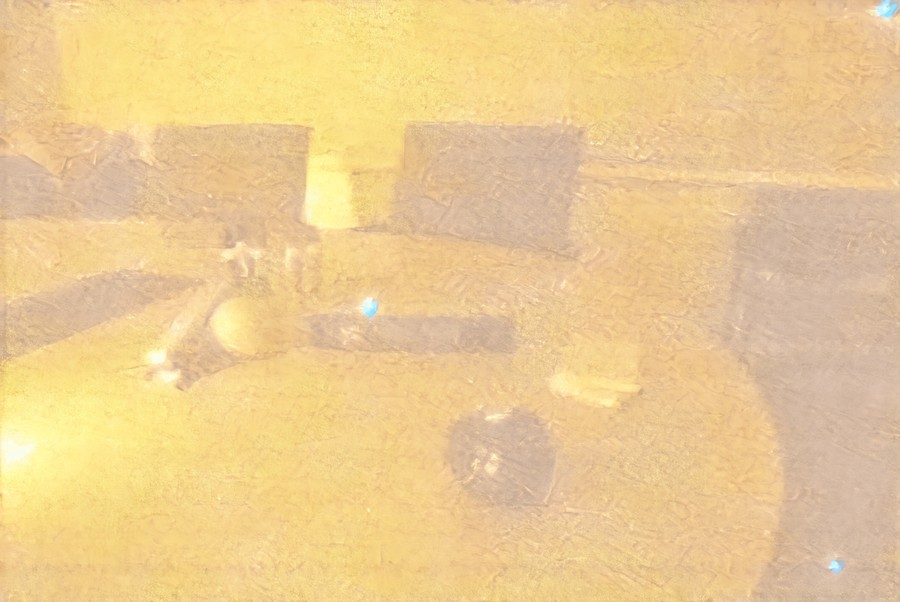
\includegraphics[width=0.32\linewidth]{bksdm_tiny} \\
    \footnotesize (a) Input, short exposure &
    \footnotesize (b) \sdtwo{} (baseline) &
    \footnotesize (c) \bksdm{} + illum. \\[2pt]
    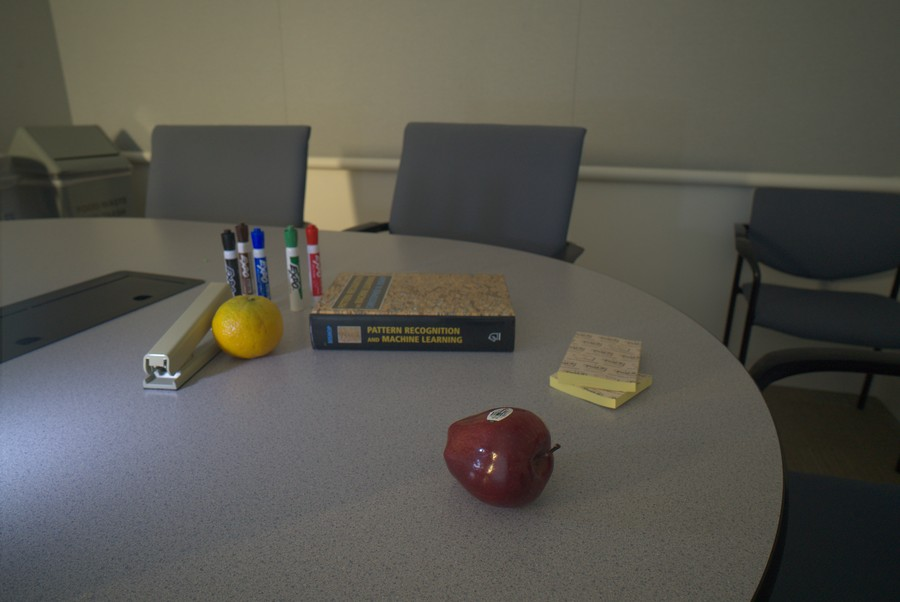
\includegraphics[width=0.32\linewidth]{reference} &
    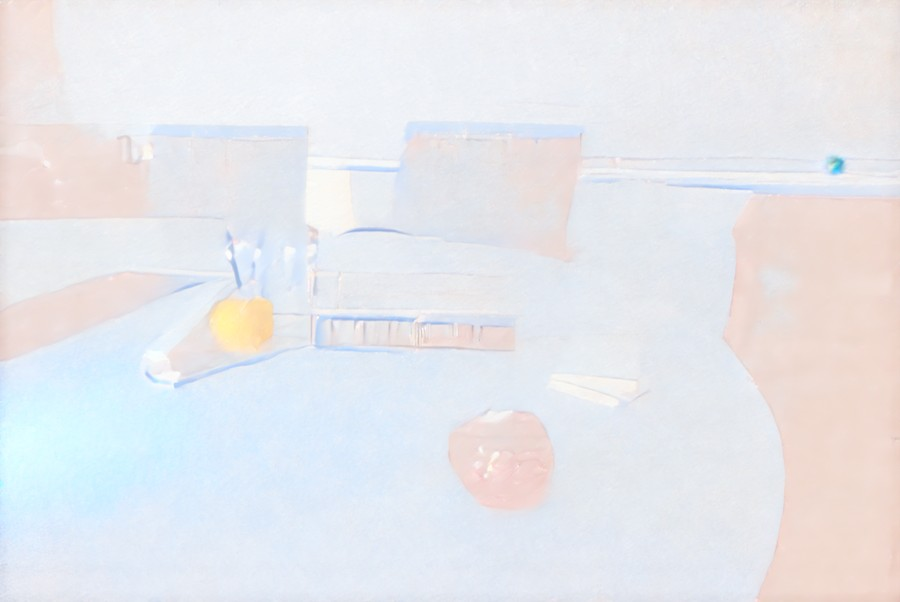
\includegraphics[width=0.32\linewidth]{tiny_sd} &
    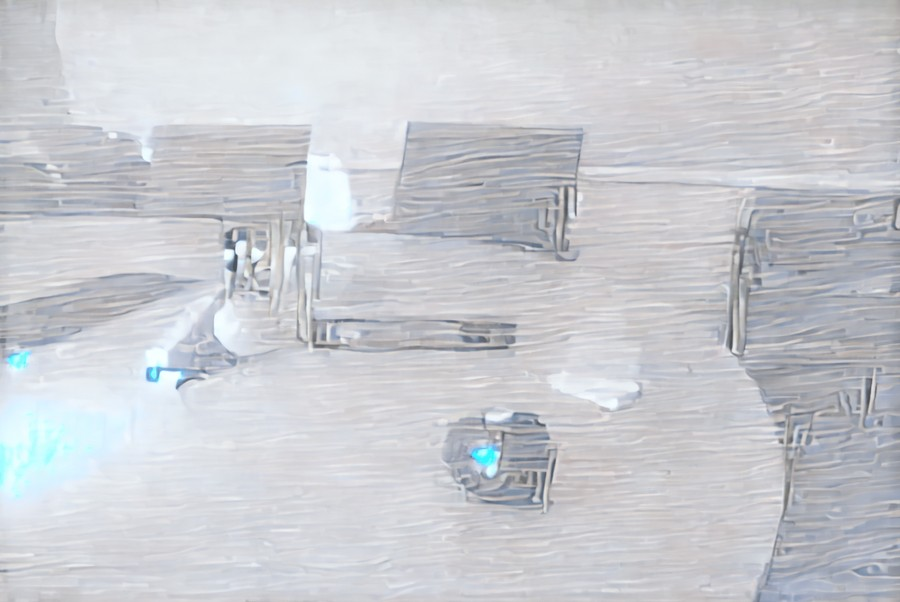
\includegraphics[width=0.32\linewidth]{sdxs512} \\
    \footnotesize (d) Reference, long exposure &
    \footnotesize (e) \tinysd{} + illum. &
    \footnotesize (f) \sdxs{} + illum.
  \end{tabular}
  \caption{Outputs on one SID test scene after 10 epochs of training for every model. The input
  is shown after the $\times300$ gain with gamma for display. The \sdtwo{} baseline keeps the
  outlines of the chairs and table but replaces the content with a washed-out, streaked texture.
  The compact models recover more of the objects, but with colour casts and lost texture.}
  \label{fig:samples}
\end{figure*}

Fig.~\ref{fig:samples} shows one test scene. The \sdtwo{} output keeps the coarse layout (the
outlines of the chairs and the table) but is washed out, nearly colourless and covered by a
hallucinated, wood-grain-like texture; the fruit and books are lost. A likely cause is that the
baseline fine-tunes 1.22B parameters at batch size 1 without learning-rate warm-up or gradient
clipping, which makes optimisation slow and unstable. The compact models, with a third of the
trainable parameters, recover more of the main objects (chairs, table, fruit, books). Their
outputs are over-exposed and colour-shifted, and \sdxs{} shows the same streak-like artefacts as
the baseline.

\subsection{Efficiency}
\label{sec:efficiency}

\begin{table}[t]
  \centering
  \caption{Efficiency on one NVIDIA A40 with $1200$\,px crops and bf16. Inference covers
  50 DDIM steps per image; compute is per U-Net call. Trainable parameters include the context
  processor.}
  \label{tab:efficiency}
  \setlength{\tabcolsep}{3pt}
  \begin{tabular}{@{}lrrrr@{}}
    \toprule
    Metric & \sdtwo{} & BK-tiny & \tinysd{} & SDXS \\
    \midrule
    Trainable params (M)  & 1218 & 417  & \textbf{413}  & 419 \\
    U-Net GFLOPs          & 813  & 496  & 495  & \textbf{428} \\
    Inference time (s)    & 2.28 & 1.37 & 1.45 & \textbf{1.31} \\
    Inference memory (GB) & 8.2  & 3.7  & \textbf{3.6}  & 3.7 \\
    Train step time (s)   & 0.59 & \textbf{0.41} & 0.42 & \textbf{0.41} \\
    Train memory (GB)     & 21.2 & \textbf{8.2}  & \textbf{8.2}  & \textbf{8.2} \\
    \bottomrule
  \end{tabular}
\end{table}

Table~\ref{tab:efficiency} shows what shrinking buys. The compact models have 66\% fewer
trainable parameters. They use 55--56\% less inference memory and 61\% less training memory,
which is within the memory of a 12\,GB consumer GPU. Inference is 36--43\% faster,
with \sdxs{} the fastest at 1.31\,s per image. Compute per U-Net call falls by 39--47\%, less
than the parameter count, because the distilled models keep the expensive high-resolution
blocks (Sec.~\ref{sec:backbones}).

\subsection{Limitations}
\label{sec:limitations}

\textbf{Short training.} Ten epochs is far from convergence, and the ranking may change with
longer training.
\textbf{Confounded comparison.} We compare the original DarkDiff with our full modification, so
the gains cannot be split between the smaller backbone and the illumination conditioning.
\textbf{No stage-1 VAE.} Without the fine-tuned residual VAE, the diffusion target is the latent
of the clean \emph{linear} image, which the pretrained decoder maps back to linear RGB, while
$\Limg$ compares against \emph{sRGB}. The two losses pull towards different images, which likely
contributes to the colour casts.
\textbf{One dataset.} We evaluate only on SID; ELD and LRD are left for future work.
